%%%%%%%%%%%%%%%%%%%%%%%%%%%%%%%%%%%%%%%%%%%%%%%%%%%%%%%%%%%%%%%%%%%%%%%
% To compile, use pdflatex file.tex

\documentclass{beamer}

%%%%%%%%%%%%%%%%%%%%%%%%%%%%%%%%%%%%%%%%%%%%%%%%%%%%%%%%%%%%%%%%%%%%%%
% Information for Beamer class.  Mostly for various themes

%\usepackage{beamerthemeRochester}

%\usetheme{Goettingen}
%\usetheme{Copenhagen}
%\usetheme{Frankfurt}
%\usetheme{Warsaw}
%\usetheme{Berlin}

 \usecolortheme{default}
\usefonttheme{default}
%\useinnertheme{rounded}
%%%%%%%%%%%%%%%%%%%%%%%%%%%%%%%%%%%%%%%%%%%%%%%%%%%%%%%%%%%%%%%%%%%%%%%
% My macros and definition go here

\usepackage{amsmath}
\usepackage{amssymb} % it does not work with MnSymbol
\usepackage{amsthm,mathrsfs}
\usepackage{enumitem}
\usepackage{bm}
\usepackage{physics}
\usepackage{multirow}
\usepackage{tabularx}
\usepackage{graphicx}
\usepackage{hyperref}
\usepackage{enumitem}
\usepackage{booktabs}
\usepackage{cite}
\usepackage{algorithm}
\usepackage{algpseudocode}
\usepackage{cprotect}
\usepackage{graphicx}
%Font used for low resolution printer, i.e 
% \usepackage[no-math]{fontspec}
% \usepackage{fourier}
% \usepackage{MnSymbol}
% \setmainfont{Linux Libertine O} 
%------------------------------
\newcommand{\RR}{\mathbb{R}}
\newcommand{\ZZ}{\mathbb{Z}}
\newcommand{\NN}{\mathbb{N}}
\newcommand{\QQ}{\mathbb{Q}}
\newcommand{\CC}{\mathbb{C}}
\newcommand{\e}{\text{e}}
\newcommand{\sumi}[2][1]{\sum\limits_{i=#1}^{#2}}
\newcommand{\sumk}[2][1]{\sum\limits_{k=#1}^{#2}}
\newcommand{\sumj}[2][1]{\sum\limits_{j=#1}^{#2}}
\newcommand{\sumx}[2][1]{\sum\limits_{x=#1}^{#2}}
\newcommand{\sumn}[2][1]{\sum\limits_{n=#1}^{#2}}
\newcommand{\prodi}[2][1]{\prod\limits_{i=#1}^{#2}}
\newcommand{\prodk}[2][1]{\prod\limits_{k=#1}^{#2}}
\newcommand{\prodj}[2][1]{\prod\limits_{j=#1}^{#2}}
\newcommand{\E}[2][]{ \mathbb{E}_{#1} \left[ #2 \right]}
\newcommand{\Var}[1]{ \text{Var} \left[ #1 \right]}
\newcommand{\Cov}[1]{ \text{Cov} \left[ #1 \right]}
\renewcommand{\P}[2][]{ \mathbb{P}_{#1} \left( #2 \right)}
\newcommand{\iidis}{\stackrel{iid}{\sim}}
\newcommand{\toP}{\stackrel{P}{\to}}
\newcommand{\toD}{\stackrel{\text{D}}{\to}}
\newcommand{\eqD}{\stackrel{\text{D}}{=}}
\newcommand{\toas}{\stackrel{\text{a.s}}{\to}}
\newcommand{\I}[1]{\mathbb 1_{\{#1\}}}
\newtheorem{thm}{Theorem}
\newtheorem{prop}{Proposition}
\newtheorem{lem}{Lemma}
\newtheorem{cor}{Corollary}

\theoremstyle{definition}
\newtheorem{defn}{Definition}
\newtheorem{eg}{Example}

\theoremstyle{remark}
\newtheorem*{rem}{Remark}
%%%%%%%%%%%%%%%%%%%%%%%%%%%%%%%%%%%%%%%%%%%%%%%%%%%%%%%%%%%%%%%%%%%%%%%
% Title page information

\title{On the Equivalence of Tests for Outliers for Pareto and Exponential Distributions}
\author{Fang Wang}
\institute{McMaster University}
\begin{document}



%%%%%%%%%%%%%%%%%%%%%%%%%%%%%%%%%%%%%%%%%%%%%%

\begin{frame}
\titlepage
\end{frame}

%%%%%%%%%%%%%%%%%%%%%%%%%%%%%%%%%%%%%%%%%%%%%%%%%%

\begin{frame}{Outline}
 \begin{enumerate}
	\item[*] Introduction \\
	\item[*] Discordancy tests  \\
	\item[*] Distribution of order statistics under monotone transformation \\
	\item[*] Power comparision and real dataset application
%\item Conclusion 
\end{enumerate}

\end{frame}
%%%%%%%%%%%%%%%%%%%%%%%%%%%%%%%%%%%%%%%%%%%%%%%%%%%%%
\begin{frame}{Introduction: Outliers}
    The outliers, in a sample of observations, is a subset of observations that appears to be inconsistent with the rest of the data and the assumption proposed
    on the dataset.
\end{frame}
%%%%%%%%%%%%%%%%%%%%%%%%%%%%%%%%%%%%%%%%%%%%%%%%%%%%

\begin{frame}{Introduction: $H_0$}
    \begin{defn}[null hypothesis of contamination model] \label{defn: H_0}
        Let $x_1,\ldots,x_n$ be a sample of $n$ observations. Then under the null hypothesis $H_0$, $x_1,\ldots,x_n$ are observations of
        $X_1,\ldots,X_n$, where $X_1,\ldots,X_n$ are independent random variables with common distribution $F$.
    \end{defn}
    
\end{frame}

%%%%%%%%%%%%%%%%%%%%%%%%%%%%%%%%%%%%%%%%%%%%%%%%%%%%

\begin{frame}{Introduction: $H_r$}
    
    \begin{defn}[slippage alternative of the contamination model] \label{defn: slippage Hr}
        Let $x_1,\ldots,x_n$ be a sample of $n$ observations with null hypothesis $x_1,\ldots,x_n$ that they are independently from a distribution $F$. Let
        $x_{(1)} < x_{(2)} <  \cdots < x_{(n)}$ be the order statistics of $x_1,\ldots,x_n$. Then under the slippage alternative $H_r$,
        the sample $x_{(1)},\ldots x_{(n-r)}$ are independent observations from distribution $F$ and $x_{(n-r+1)},\ldots, x_{(n)}$ are independent observations
        from distribution $\overline F$ with $F \neq \overline F$.
    \end{defn}
\end{frame}
%%%%%%%%%%%%%%%%%%%%%%%%%%%%%%%%%%%%%%%%%%%%%%%%%%%%

%%%%%%%%%%%%%%%%%%%%%%%%%%%%%%%%%%%%%%%%%%%%%%%%%%%%
\begin{frame}{Contamination Model }
    \begin{figure}
        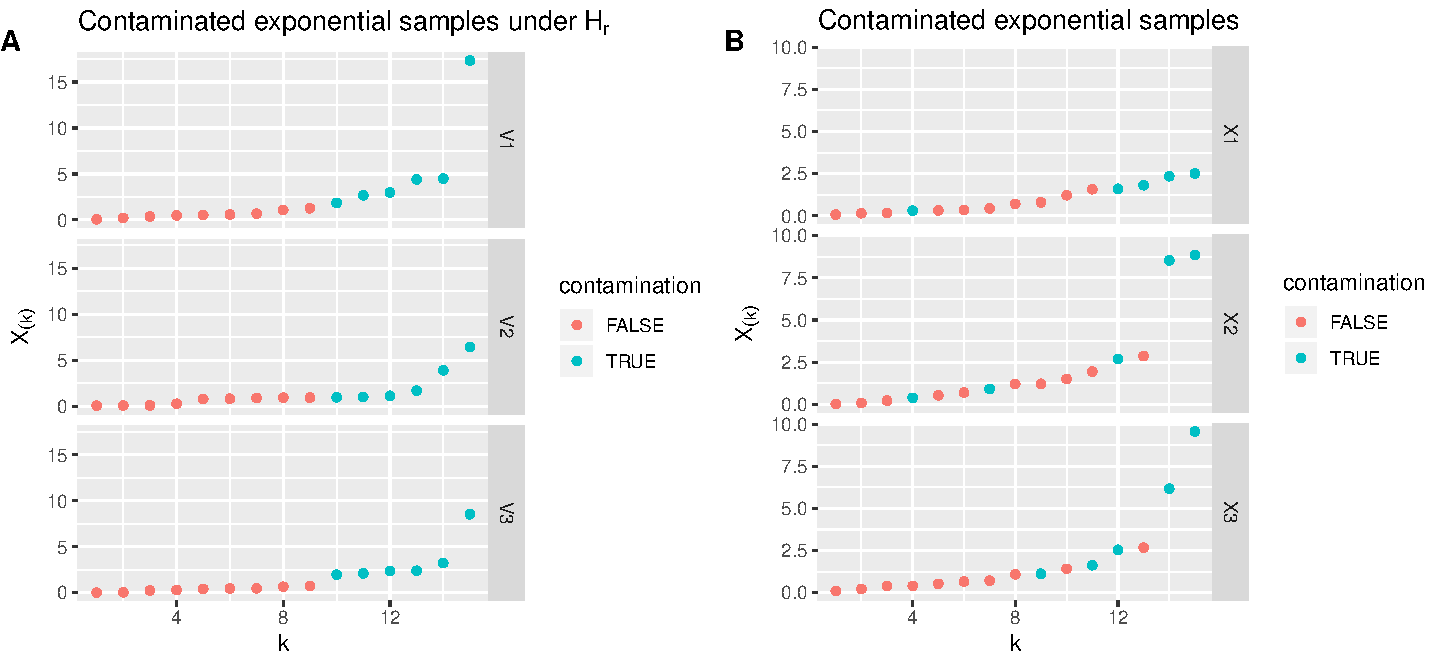
\includegraphics[scale = 0.4]{plot_0.pdf}
    \end{figure}
    \textbf{A}: Contaminated samples with $H_r$ \\
    \textbf{B}: Contaminated samples without $H_r$
\end{frame}

%%%%%%%%%%%%%%%%%%%%%%%%%%%%%%%%%%%%%%%%%%%%%%%%%%%%
\begin{frame}{Exponential Distribution}
    \begin{defn}[Exponential distribution]
        A random variable $X$ follows exponential distribution with mean parameter $\theta > 0$ if it has pdf of
        \[ 
            f(x) = \frac{1}{\theta} e^{-x/\theta}, \quad x >0
            \]
            and we denoted it by $X \sim \mathrm{Exp}(\theta)$.
        \end{defn}
    \end{frame}
    
    %%%%%%%%%%%%%%%%%%%%%%%%%%%%%%%%%%%%%%%%%%%%%%%%%%%%
    \begin{frame}{Poission Process}
       \begin{itemize}
           \item[*] Let $N(t)$ be a Poisson process with rate parameter $1/\theta$, and stage space $\{0,1\}$,
           then the sojourn time of $N_t$ follows $\mathrm{Exp}(\theta)$ distribution.
            \item[*] If $Y_1,\ldots,Y_k$ are iid exponential samples, they are also sojourn times of some Poisson processes $N_1,\ldots,N_k$.
            \item[*] Let $N = N_1+ \ldots+N_k$, then $Y_{(i)} - Y_{(i-1)}$ are sojourn time of $N$ in stage $i_1$ 
       \end{itemize}
    \end{frame}
        %%%%%%%%%%%%%%%%%%%%%%%%%%%%%%%%%%%%%%%%%%%%%%%%%%%%
        
        
\begin{frame}{Pareto Distribution}
    \begin{defn}[Pareto distribution]
        A random variable $X$ follows $\mathrm{Pareto}(\alpha,\theta)$ distribution if its pdf is given by
        \[ 
            f(x;\alpha,\theta) = \frac{\alpha \theta^{\alpha}}{x^{\alpha +1}}, \quad x \geqslant \theta >0
            \]
            where $\theta$ and $\alpha$ are both positive parameters.
        \end{defn}

        \begin{rem} \label{lem: log of Pareto is exp}
            Suppose $X \sim \mathrm{Pareto}(\alpha,\theta)$ and $Y = \log(X/\theta)$. Then, $Y \sim \mathrm{Exp}(\alpha)$.
        \end{rem}
    \end{frame}
%%%%%%%%%%%%%%%%%%%%%%%%%%%%%%%%%%%%%%%%%%%%%%%%%%%%





\begin{frame}{$H_r$ for Exponential and Pareto Distributions }
    Let $\alpha$ and $\theta$ be two positive real numbers and $b \in (0,1)$.
    \begin{description}
        \item[Exponential Case ] $F$ is $\text{Exp}(\theta)$ and $\overline{F}$ is $\text{Exp}(\theta/b)$ \\
        \item[Pareto Case ] $F$ is $\text{Pareto}(\alpha, \theta)$, $\overline{F}$ is $\text{Pareto}(\alpha b, \theta)$
    \end{description}

\end{frame}

%%%%%%%%%%%%%%%%%%%%%%%%%%%%%%%%%%%%%%%%%%%%%%%%%%%

\begin{frame}{Simulate Exponential Sample Under $H_r$}
    \begin{enumerate}
        \item[1] Generate $n-r$ observations from $F$ and $r$ observation from $\overline F$.
        \item[2] Combined total $n$ observations into a single observation $\mathbf x$ 
        \item[3] Accept $\mathbf x$ if it satisfies $H_r$.
    \end{enumerate}

    If $F$ is $\text{Exp}(\theta)$ and $\overline{F}$ is $\text{Exp}(\theta/b)$,the acceptance probability is
    \begin{align*}
        \P{\text{Acceptance}} &= \P{\max\{X_{1},\ldots, X_{n-r}\} < \min\{X_{n-r+1},\ldots, X_{n}\}}
        \\
        &= rb B(rb, n-r+1),
    \end{align*}
    where $B(r,s)$ is the complete beta function.
\end{frame}

%%%%%%%%%%%%%%%%%%%%%%%%%%%%%%%%%%%%%%%%%%%%%%%%%%%%

\begin{frame}{Acceptance Probability for Various Parameters}
        \begin{figure}
            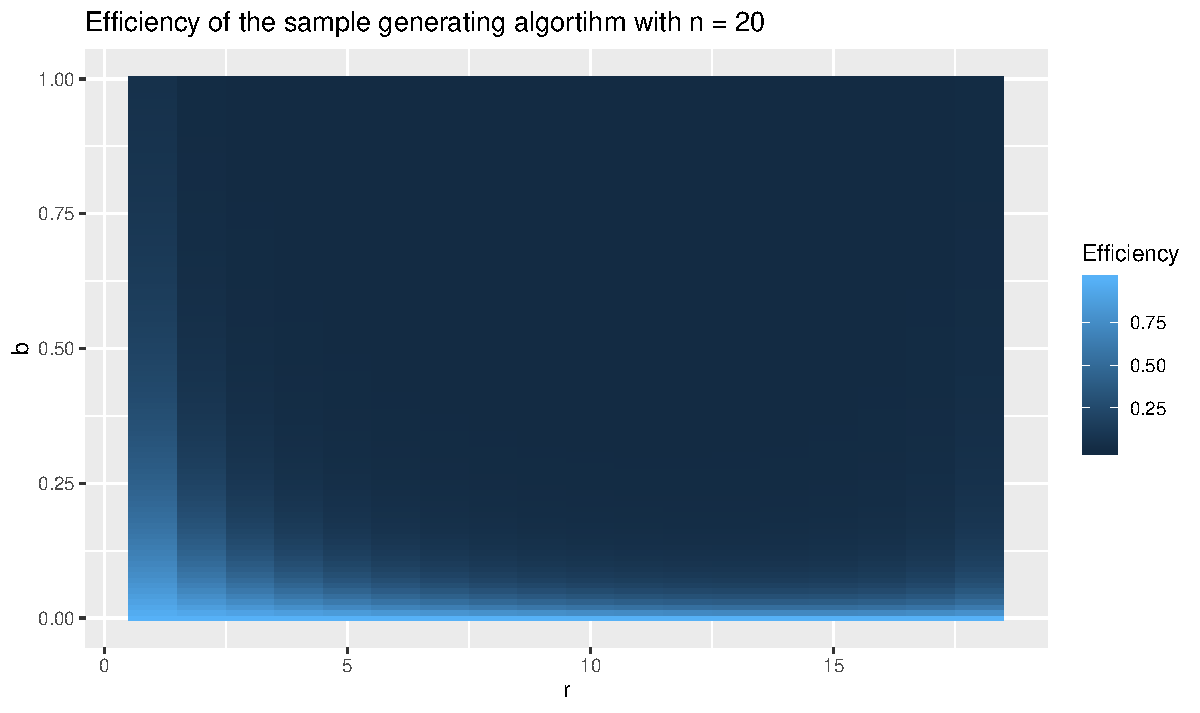
\includegraphics[scale = 0.5]{plot_eff.pdf}
        \end{figure}
    \end{frame}
    
%%%%%%%%%%%%%%%%%%%%%%%%%%%%%%%%%%%%%%%%%%%%%%%%%%%%%

\begin{frame}{Discordancy Test Statistics for Exponential $H_r$}

    \begin{align*}
        D_r(\mathbf X) &= \frac{X_{(n)} - X_{(n-r)}}{X_{(n)}},  \\
        R_r(\mathbf X) &= \frac{X_{(n-r)} - X_{(1)}}{X_{(n)} - X_{(n-r+1)}}, \\
        Z_r(\mathbf X) &= \frac{X_{(n-r)} -X_{(1)}}{\sum_{j = n - r + 1}^n X_{(j)} - X_{(1)}}.
    \end{align*}
\end{frame}

%%%%%%%%%%%%%%%%%%%%%%%%%%%%%%%%%%%%%%%%%%%%%%%%%%%%%

\begin{frame}{Discordancy Test Statistics for Pareto $H_r$}
    
    \begin{align*}
        \tilde D_r(\mathbf Y) &= \frac{\ln(Y_{(n)}) - \ln(Y_{(n-r)})}{\ln(Y_{(n)})}, \label{eqn: modified Dr} \\
        \tilde R_r(\mathbf Y)  &= \frac{\ln(Y_{(n-r)}) - \ln(X_{(1)})}{\ln(Y_{(n)}) - \ln(Y_{(n-r+1)})}, \\
        \tilde Z_r(\mathbf Y) &= \frac{\ln(Y_{(n-r)}) - \ln(Y_{(1)})}{\sum_{j = n - r + 1}^n \ln(Y_{(j)}) - \ln(Y_{(1)})}.
    \end{align*}
\end{frame}

%%%%%%%%%%%%%%%%%%%%%%%%%%%%%%%%%%%%%%%%%%%%%%%%%%%%%

\begin{frame}{Distributional Result}
    
    \begin{thm}
        Let $X_1,X_2,\ldots, X_n$ be continuous random variables with density $f_1,\ldots, f_n$, respectively, where $f_i$ has the same support $(a,b)$ with $-\infty \leqslant a < b \leqslant \infty$. Let
        $g_1,\ldots,g_n$ be a collection of strictly increasing differentiable functions with domain $(a,b)$ and range $(c,d) \subseteq \RR$.
        Define random variable $Y_i = g_i(X_{(i)}),$ for $i =1,\ldots,n$.
    Then, the joint pdf of $Y_1,\ldots Y_n$ is given by
    {\small
    \[ 
        f_{Y_1,\ldots,Y_n}(y_1,\ldots, y_n) = \begin{cases}
            n!\prodi{n} \abs{ \dv{g_i^{-1}}{y}}  f_i(y_i), & c < y_1 < y_2 <\cdots < y_n < d
            \\
            0, & \text{elsewhere.}
        \end{cases}
        \]}
    \end{thm}
\end{frame}

%%%%%%%%%%%%%%%%%%%%%%%%%%%%%%%%%%%%%%%%%%%%%%%%%%%%%

\begin{frame}
    \begin{cor} \label{cor: distribution of log Pareto OS}
        Let $X_1, \ldots X_n$ and $E_1,\ldots, E_n$ be independent random variables with $ X_k \sim \mathrm{Pareto}(\alpha_k,\theta_k)$ and
        $E_k \sim \mathrm{Exp}(\alpha_k)$ for $k =1,\ldots,n$. Let $Y_k = E_{(k)}$ and $U_k = \ln(X_{(k)}/\theta_k)$, for $k =1,\ldots,n$.
        Then the random vector $\mathbf U =(U_1,\ldots, U_n)$ has the same distribution as $\mathbf Y = (Y_1,\ldots,Y_n)$.
    \end{cor}
    \begin{rem}
        The conclusion holds under $H_r$.
    \end{rem}
\end{frame}

%%%%%%%%%%%%%%%%%%%%%%%%%%%%%%%%%%%%%%%%%%%%%%%%%%%%%

\begin{frame}{Equivalence of Tests}
    \begin{itemize}
        \item[*] $D_r(\mathbf Y) \eqD \tilde D_r(\mathbf X)$, $Z_r(\mathbf Y) \eqD \tilde Z_r(\mathbf X)$ and $R_r(\mathbf Y) \eqD \tilde R_r(\mathbf X)$ under $H_r$.
        \item[*] Statistics tests based on $D_r$, $R_r$ and $Z_r$ would have the same power and critical values as $\tilde D_r$, $\tilde R_r$ and $\tilde Z_r$, respectively.
        \item[*] statistics used for testing slippage alternative hypothesis of exponential samples can be easily adapted to test for the Pareto case 
    \end{itemize}
\end{frame}

%%%%%%%%%%%%%%%%%%%%%%%%%%%%%%%%%%%%%%%%%%%%%%%%%%%%%

\begin{frame}{Power of Tests}
    \begin{figure}
        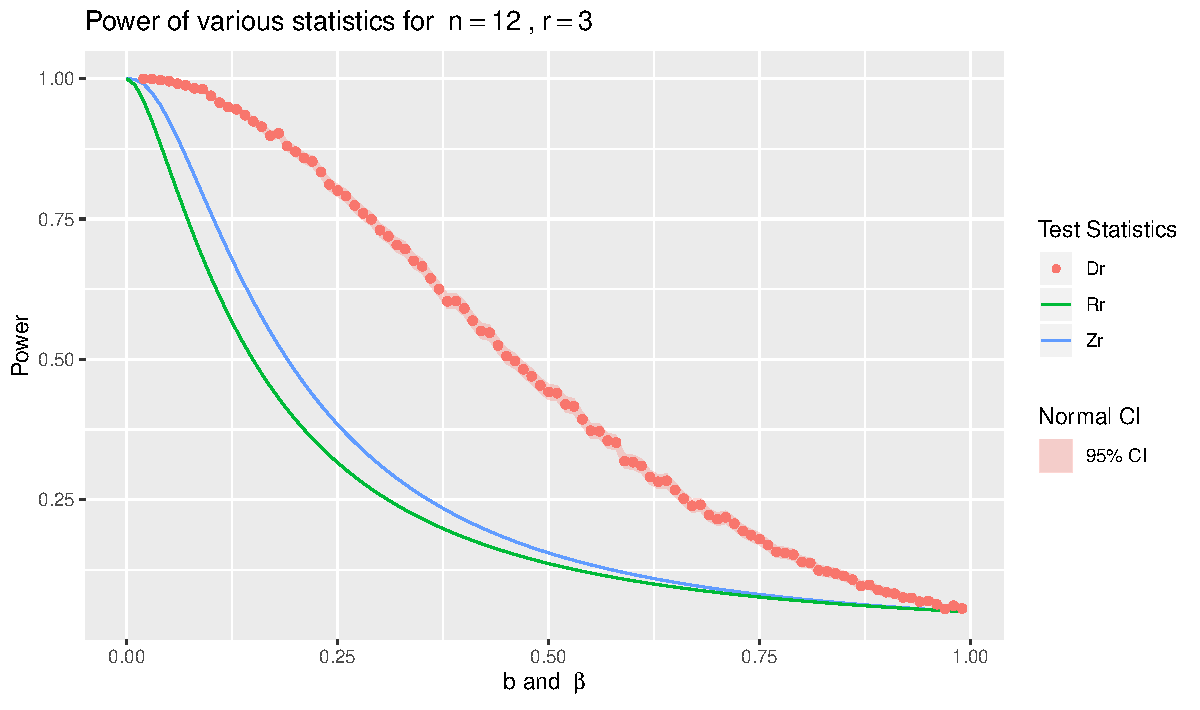
\includegraphics[scale = 0.5]{plot_5.pdf}
    \end{figure}
\end{frame}
%%%%%%%%%%%%%%%%%%%%%%%%%%%%%%%%%%%%%%%%%%%%%%%%%%%%%
\begin{frame}{Real Dataset Application }
    \begin{itemize}
        \item[*] Haberman’s survival dataset
        \item[*] Mean of parameter of two distribution: $\theta_1 = 2.80 , \theta_2 = 7.46,$
        \item[*] Sample size: $N_1 = 85, N_2 = 244$
        \item[*] Estimated power: $\hat{\gamma(D_r)} = 0.475, \hat{\gamma(Z_r)} = 0.455, \hat{\gamma(R_r)} = 0.28$.   
    \end{itemize}
    \begin{figure}
        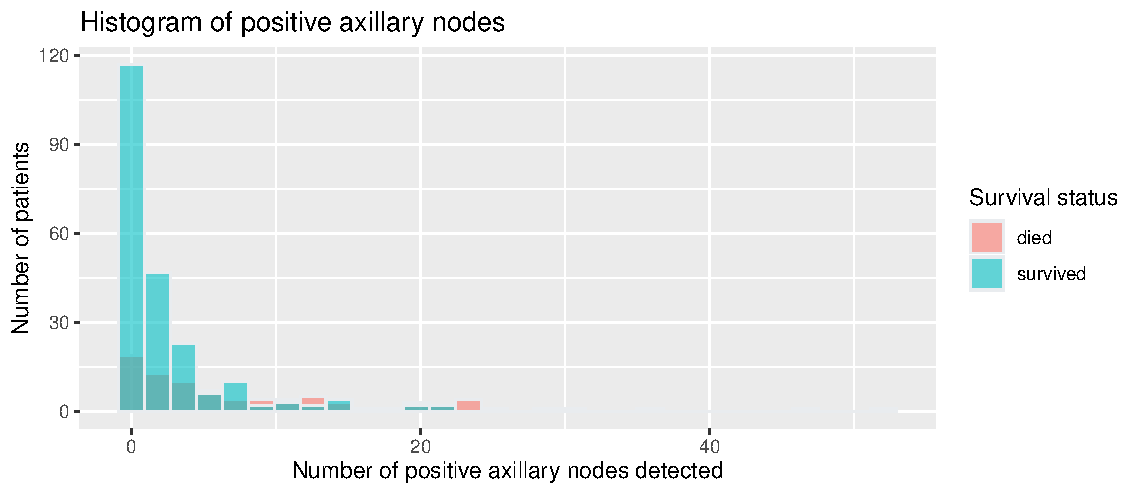
\includegraphics[scale = 0.5]{plot_cancer.pdf}
    \end{figure}
\end{frame}



%%%%%%%%%%%%%%%%%%%%%%%%%%%%%%%%%%%%%%%%%%%%%%%%%%%%%
\end{document}